\documentclass{beamer}

\usetheme{Warsaw}
\usecolortheme{seahorse}
\setbeamertemplate{navigation symbols}{}
\setbeamertemplate{bibliography item}{\insertbiblabel}
\setbeamertemplate{caption}{\raggedright\scriptsize\insertcaption\par}
\setbeamercolor{background canvas}{bg=}
\usepackage{beamerthemesplit}
\usepackage{pgf}
\usepackage{epsfig}
\usepackage{epstopdf}
\usepackage{graphicx}
\usepackage{slashbox}
\usepackage{url}
\usepackage{listings}
\usepackage{polski}
\usepackage[utf8]{inputenc}
\usepackage[absolute,overlay]{textpos}
\usepackage{graphicx}
\newcommand{\IR}{\bbold R}
\def\Rset{\mathbb{R}}
\def\Zset{\mathbb{Z}}
\newcommand{\refbr}[1]{(\ref{#1})}
\newcommand{\beq}{\begin{equation}}
\newcommand{\eeq}{\end{equation}}
\newcommand{\und}[1]{\underline{#1}}
\newcommand\pro{\item[$+$]}
\newcommand\con{\item[$-$]}
\newcounter{saveenumi}
\newcommand{\seti}{\setcounter{saveenumi}{\value{enumi}}}
\newcommand{\conti}{\setcounter{enumi}{\value{saveenumi}}}
\lstset{
    numbers=left,
    breaklines=true,
    tabsize=2,
	numberstyle=\color{gray}\footnotesize,
    basicstyle=\small\ttfamily,
}
% \AtBeginSection{
%   \begin{frame}
%   \vfill
%   \centering
%   \begin{beamercolorbox}[sep=8pt,center,shadow=true,rounded=true]{title}
%     \usebeamerfont{title}\insertsectionhead\par%
%   \end{beamercolorbox}
%   \vfill
%   \end{frame}
% }

\hypersetup{
   pdftitle={Oprogramowanie do gier opartych o planszę w postaci szachownicy},
   pdfauthor={Jakub Ostrzołek},
   pdfborder={0 0 0}
}

\title[Silnik gier opartych o szachownicę \insertframenumber/\inserttotalframenumber]{
   Projekt i wykonanie oprogramowania do gier planszowych opartych
   o planszę postaci szachownicy -- podejście w oparciu o dedykowany
   język dziedzinowy.}
\author[Jakub Ostrzołek]{\textbf{Jakub Ostrzołek} \\%
\footnotesize Promotor: dr inż. Patryk Chaber}
\institute{Instytut Automatyki i Informatyki Stosowanej\\%
Politechnika Warszawska}

\begin{document}

\frame{\titlepage}

\frame{\tableofcontents\frametitle{Plan prezentacji}}

\section{Cel pracy}

\begin{frame}
	\frametitle{Cele pracy}
	\begin{enumerate}
		\item opracowanie języka dziedzinowego do opisywania zasad gier planszowych opartych o szachownicę
		\item implementacja silnika gry
		      \begin{itemize}
			      \item potrafi interpretować zasady w ww. języku
			      \item pozwala na rozgrywkę dwóch osób
		      \end{itemize}
		\item stworzenie interfejsu użytkownika
	\end{enumerate}
\end{frame}

\section{Tematyka pracy}

\begin{frame}
	\frametitle{Język -- wstępne założenia}
	\begin{itemize}
		\item opisuje gry 2-osobowe, turowe, deterministyczne
		\item możliwie nieskomplikowany
		\item wymaga rozumienia podstawowych zasad programowania
		\item zwięzły
		\item pozwala wyrazić zasady min. 3 gier -- tradycyjne szachy, Halma, Dōbutsu shōgi
	\end{itemize}
\end{frame}

\begin{frame}
	\frametitle{Halma}
	\begin{columns}
		\begin{column}{.48\textwidth}
			\begin{itemize}
				\item Cel -- ustawić wszystkie piony na polu startowym przeciwnika
				\item Poruszanie o 1 po  krawędziach kwadratu
				\item Przeskakiwanie przez 1 piona po krawędziach kwadratu (dozwolone łączenie wiele na raz)
			\end{itemize}
		\end{column}%
		\hfill
		\begin{column}{.60\textwidth}
			\begin{figure}
				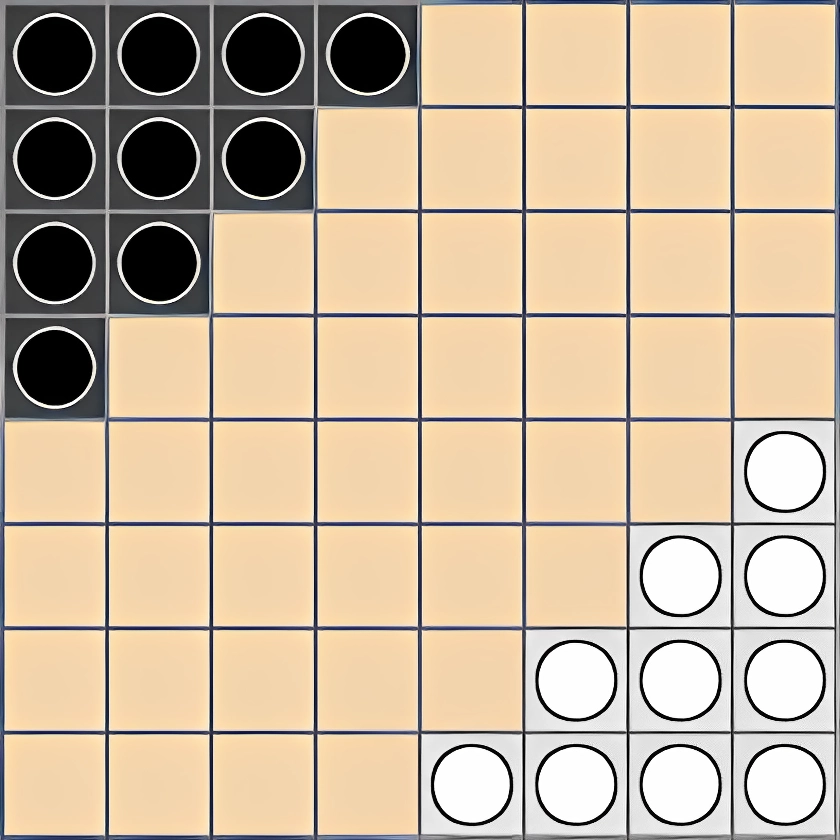
\includegraphics[height=4.5cm]{halma.png}
				\centering
				\caption{\url{https://brainking.com/en/GameRules?tp=33}}
			\end{figure}
		\end{column}
	\end{columns}
\end{frame}

\begin{frame}
	\frametitle{Dōbutsu shōgi}
	\begin{columns}
		\begin{column}{.48\textwidth}
			\begin{itemize}
				\item Cel -- zbić lwa przeciwnika lub przejść lwem na stronę przeciwnika
				\item Poruszanie zgodnie z oznaczeniami na figurach
				\item Promocja kurczaka do kury
				\item Możliwość kładzenia zbitych figur przeciwnika
			\end{itemize}
		\end{column}%
		\hfill
		\begin{column}{.60\textwidth}
			\begin{figure}
				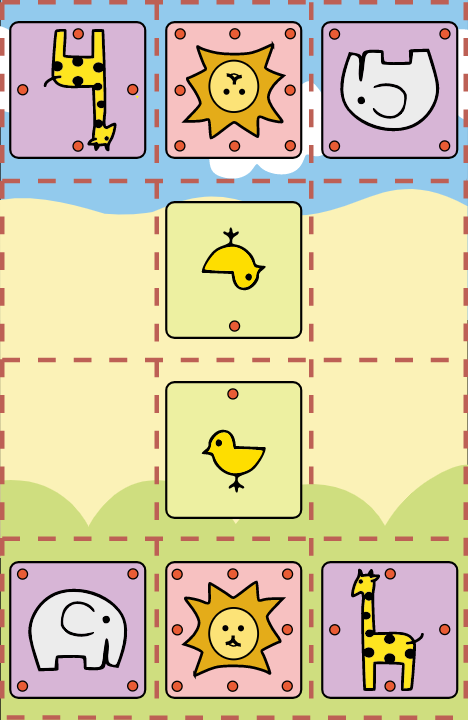
\includegraphics[height=4.5cm]{dobutsu-shogi.png}
				\centering
				\caption{\url{https://www.pychess.org/variants/dobutsu}}
			\end{figure}
		\end{column}
	\end{columns}
\end{frame}

\begin{frame}
	\frametitle{Silnik gry}
	\begin{columns}
		\begin{column}{.50\textwidth}
			Silnik gry -- automat
			\begin{itemize}
				\item odseparowany od modułu dekodującego zasady
				\item inicjalizowany stanem początkowym pochodzącym z modułu dekodującego zasady
				\item dla każdego stanu generuje możliwe przejścia
				\item dobrze przetestowany
			\end{itemize}
		\end{column}%
		\hfill
		\begin{column}{.50\textwidth}
			\begin{figure}
				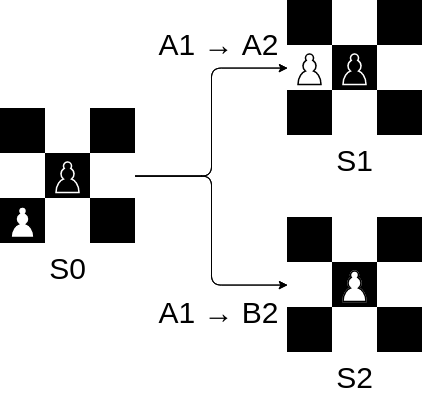
\includegraphics[width=4.5cm]{stany.png}
				\centering
			\end{figure}
		\end{column}
	\end{columns}
\end{frame}

\begin{frame}
	\frametitle{Interfejs użytkownika}
	\begin{itemize}
		\item Tematycznie najmniej istotna część projektu
		\item Wersja minimalna
		      \begin{itemize}
			      \item interfejs terminalowy
			      \item rozgrywka na jednym urządzeniu
		      \end{itemize}
		\item Wersja docelowa
		      \begin{itemize}
			      \item interfejs w przeglądarce internetowej
			      \item komunikacja z serwerem, na którym działa silnik gry (po protokole HTTP/WS)
			      \item rozgrywka poprzez 2 urządzenia
		      \end{itemize}
	\end{itemize}
\end{frame}


\section{Istniejące rozwiązania}

\begin{frame}
	\frametitle{BGD -- BoardGameDescription\cite{BGD}}
	\begin{itemize}
		\item Język opisu gier planszowych (szeroki zakres)
		\item Główny cel: możliwość opisu jak największej liczby gier
		\item Opis gry za pomocą abstrakcyjnych elementów składowych (np. obiekt, lokacja, widoczność)
		\item Mało zwięzły (np. implementacja Chińczyka -- 400 linii, Manilla -- 1100 linii)
		\item Brak udogodnień znanych z języków programowania (np. pętle, listy)
	\end{itemize}
\end{frame}

\begin{frame}
	\frametitle{RAS -- Rule Automation System\cite{RAS}}
	\begin{itemize}
		\item Język opisu gier karcianych
		\item Główny cel: używanie przez ludzi niezaznajomionych z programowaniem
		\item Ograniczony tylko do gier karcianych
		\item Brak udogodnień znanych z języków programowania (np. pętle, listy)
	\end{itemize}
\end{frame}

\begin{frame}
	\frametitle{Metagame\cite{metagame}}
	\begin{itemize}
		\item Język opisu gier opartych o szachownicę
		\item Główny cel: dokładny opis gier na potrzeby zadań SI
		\item Bardzo rozbudowany, wiele elementów składowych języka
		\item Skomplikowany w pisaniu i rozumieniu
	\end{itemize}
\end{frame}

\begin{frame}
	\frametitle{GDL -- Game Description Language\cite{GDL}}
	\begin{itemize}
		\item Język opisu gier planszowych (szeroki zakres)
		\item Główny cel: opis jak największej liczby gier do zadań SI
		\item Podobny do Prologa -- predykaty głównym budulcem zasad
		\item Bardzo elastyczny, przy tym mało skomplikowany
		\item Brak wbudowanych konceptów gier planszowych (takich jak: plansza, gracz)
		\item Brak wbudowanych operacji arytmetycznych
	\end{itemize}
\end{frame}

\begin{frame}
	\frametitle{Wnioski}
	\begin{itemize}
		\item Istnieją rozwiązania spełniające cele mojego projektu
		\item Skupiają się na wykorzystaniu w zadaniach SI
		\item Mało przyjazne dla użytkownika definiującego zasady
		\item Wymagają doświadczonego programisty do opisu zasad
	\end{itemize}
\end{frame}

\section{Zadania pracy}

\begin{frame}
	\frametitle{Język -- elementy}
	Elementy języka:
	\begin{itemize}
		\item definicja planszy (rozmiar)
		\item stan początkowy (ustawienie figur na planszy)
		\item definicja typów figur
		      \begin{itemize}
			      \item generatory ruchu (funkcje typu: {\tt pozycja $\rightarrow$ []pozycja})
			      \item akcje (funkcje typu: {\tt pozycja $\rightarrow$ void})
		      \end{itemize}
		\item walidatory stanu gry po ruchu (funkcje typu: {\tt ruch $\rightarrow$ bool})
		\item predykat zakończenia gry + wybór zwycięzcy
		% \item funkcja przebiegu rundy
		\item bieżący stan gry dostępny z każdej funkcji (tylko do odczytu)
		\item kilka funkcji wbudowanych modyfikujących stan gry (np. {\tt capture, move})
	\end{itemize}
\end{frame}

\begin{frame}
	\frametitle{HCL bazą języka}
	Istniejący format HCL jako baza języka
	\begin{itemize}
		\item sprawdzony i znany format używany m. in. w Terraformie\footnotemark
		\item zawiera elementy standardowych języków programowania:
		      \begin{itemize}
			      \item ewaluacja wyrażeń arytmetycznych i logicznych
			      \item wykonywanie funkcji wbudowanych
			      \item pętle w postaci ,,list/obiektów składanych'' (ang. list/object comprehension)
		      \end{itemize}
		\item oficjalny dodatek {\tt userfunc} umożliwia definicję funkcji przez użytkownika
		\item zwięzły i czytelny kod
	\end{itemize}
	\footnotetext{Terraform -- narzędzie do zarządzania infrastrukturą komputerową w modelu infrastruktura jako kod (ang. IaC -- Infrastructure as Code)}
\end{frame}

\begin{frame}%[allowframebreaks]
	\frametitle{Pozostałe ustalenia}
	\begin{itemize}
		% \item Język:
		%       \begin{itemize}
		% 	      \item opracowanie wstępnego pliku zasad przed pracami nad silnikiem i modyfikacja w miarę potrzeb
		% 	      \item moduł dekodujący, sprowadzający do obiektów domenowych używanych w silniku
		% 	      \item testy plików zasad w postaci testów integracyjnych
		%       \end{itemize}
		\item Silnik:
		      \begin{itemize}
			      \item język: Go (w nim jest napisany parser HCL)
			    %   \item testy jednostkowe silnika w odosobnieniu od modułu dekodującego zasady
			      \item komunikacja między obiektami za pomocą zdarzeń % (łatwa implementacja cofania ruchów)
		      \end{itemize}
		    %   \framebreak
		\item Interfejs użytkownika:
		      \begin{itemize}
			      \item początkowo tymczasowy interfejs terminalowy
			      \item docelowo interfejs w przeglądarce
			      \item TypeScript + React
			      \item komunikacja z silnikiem za pomocą protokołu HTTP oraz WebSocket
		      \end{itemize}
	\end{itemize}
\end{frame}

\section{Dotychczasowe wyniki pracy}

\begin{frame}
	\frametitle{Dotychczasowe wyniki pracy}
	\begin{itemize}
		\item Opisane wszystkie 3 gry w plikach z zasadami
		\item Silnik potrafiący poprawnie interpretować powyższe pliki
		\item Pokrycie testami silnika na poziomie 56,2\%
		\item Tymczasowy interfejs terminalowy gotowy
		\item Rozpoczęcie prac nad interfejsem w przeglądarce
	\end{itemize}
\end{frame}

\begin{frame}[fragile]
	\frametitle{Język -- przykładowy kod (definicja typu figury)}

	\begin{lstlisting}
piece_type "king" {
	motion {
		generator = "motion_castling"
		actions   = ["displace_rook_after_castling"]
	}
	motion {
		generator = "motion_neighbours"
	}
}
	\end{lstlisting}
\end{frame}

\begin{frame}[fragile]
	\frametitle{Język -- przykładowy kod (generator ruchu)}

	\begin{lstlisting}
composite_function "motion_neighbours" {
  params = [square, piece]
  result = {
    offsets = [
      [0, 1], [1, 0], [0, -1], [-1, 0],
      [1, 1], [1, -1], [-1, 1], [-1, -1]
    ]
    dests = [for offset in offsets : get_square_relative(square, offset)]
    return = [
      for dest in filternulls(dests) : dest
      if !belongs_to(piece.color, dest)
    ]
  }
}
	\end{lstlisting}
\end{frame}

\begin{frame}
	\frametitle{Interfejs terminalowy -- szachy}
	\centering
	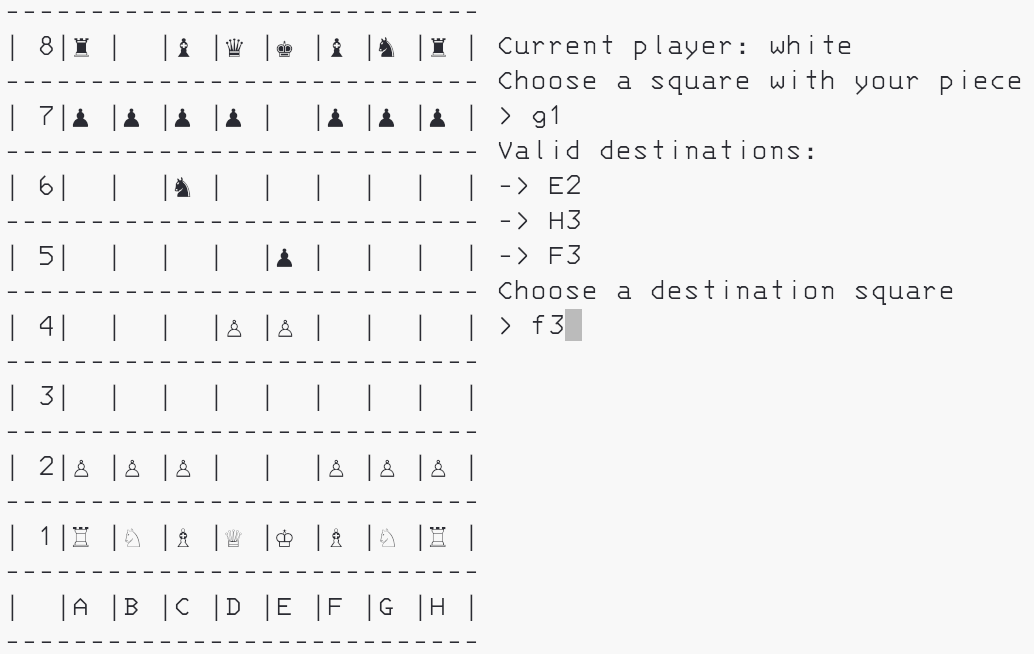
\includegraphics[width=0.95\textwidth]{chess-terminal.png}
\end{frame}

\begin{frame}
	\frametitle{Interfejs terminalowy -- Halma}
	\centering
	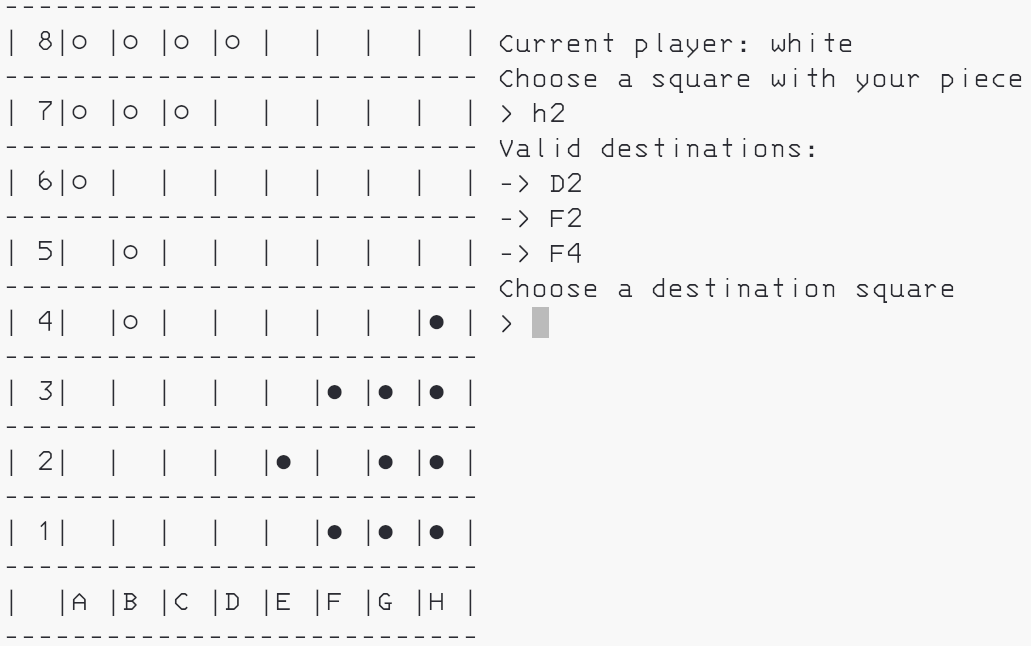
\includegraphics[width=0.95\textwidth]{halma-terminal.png}
\end{frame}

\begin{frame}
	\frametitle{Interfejs terminalowy -- Dōbutsu shōgi}
	\centering
	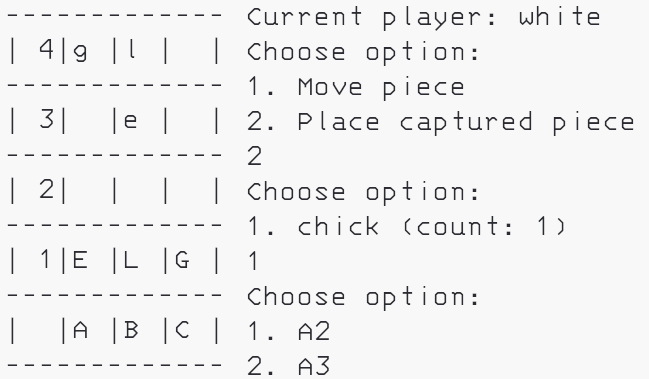
\includegraphics[width=0.95\textwidth]{dobutsu-shogi-terminal.png}
\end{frame}

\begin{frame}
	\frametitle{Interfejs w przeglądarce -- szachy}
	\centering
	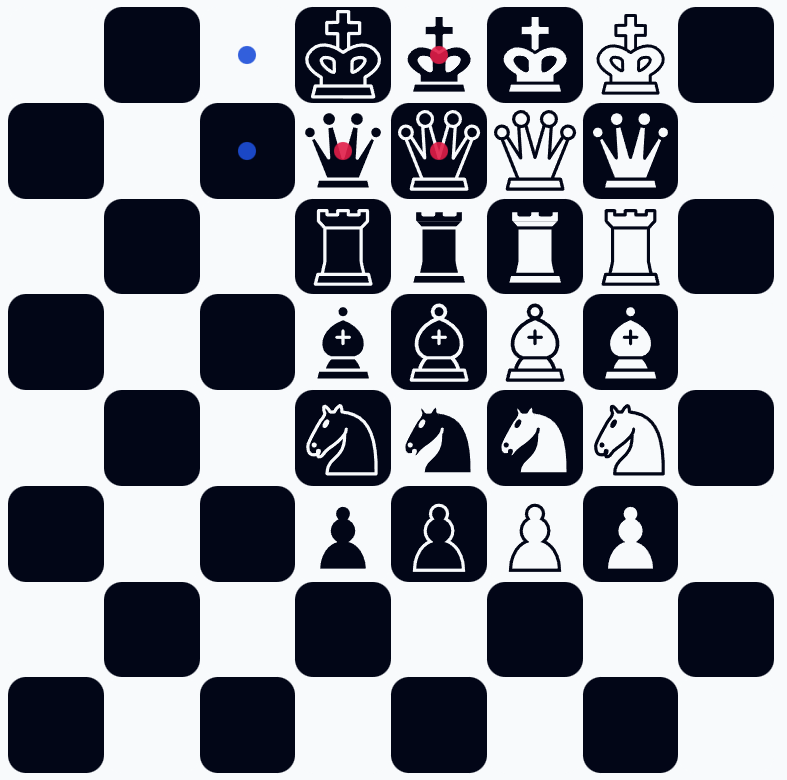
\includegraphics[height=0.85\textheight]{chess-browser.png}
\end{frame}

\section{Plan przyszłych prac}

\begin{frame}
	\frametitle{Program minimum (gotowy)}
	\begin{itemize}
		\item Opracowanie języka dziedzinowego, bazującego na HCL, do opisywania zasad dwuosobowych gier planszowych opartych o szachownicę
		\item Język musi pozwalać na opisanie zasad:
		      \begin{itemize}
			      \item standardowych szachów
			      \item gry Dōbutsu Shōgi
			      \item gry Halma
		      \end{itemize}
		\item Projekt i implementacja silnika gry, będącego interpreterem ww. języka,
		\item Stworzenie interfejsu użytkownika, pozwalającego na prowadzenie rozgrywki dwóch osób
	\end{itemize}
\end{frame}

\begin{frame}
	\frametitle{Plan przyszłych prac}
	\begin{itemize}
		\item Październik:
		      \begin{itemize}
			      \item Stworzyć serwer HTTP/WS do interakcji z silnikiem
			      \item Połączyć interfejs w przeglądarce z ww. serwerem
		      \end{itemize}
		\item Listopad:
		      \begin{itemize}
			      \item Dodać możliwość gry na wielu urządzeniach
			      \item Rozszerzyć plik z zasadami o możliwość konfiguracji wyglądu figur
		      \end{itemize}
		\item Grudzień i Styczeń
		      \begin{itemize}
			      \item Napisać pracę inżynierską
		      \end{itemize}
	\end{itemize}
\end{frame}

\begin{frame}
	\frametitle{Dodatkowe zagadnienia do rozwiązania}
	\begin{itemize}
		\item Zwiększyć poziom pokrycia kodu testami
		\item Zautomatyzować budowanie projektu (konteneryzacja)
		\item Wdrożyć projekt na wybraną usługę chmurową
		\item Dodać edytor tekstowy zasad do interfejsu w przeglądarce
		\item Dodać przyjazny edytor graficzny zasad do interfejsu w przeglądarce
	\end{itemize}
\end{frame}

\section{Podsumowanie}

\begin{frame}
	\frametitle{Podsumowanie}

	\begin{itemize}
		\item Język dziedzinowy do generowania gier planszowych opartych o szachownicę
		\item Język bazuje na HCL, charakteryzuje się prostotą pisania i modyfikowania reguł oraz zwięzłością
		\item Opis zasad gry za pomocą funkcji ułatwia rozumienie kodu
	\end{itemize}
\end{frame}

\begin{frame}[allowframebreaks,noframenumbering]
	\frametitle{Bibliografia}
	\bibliographystyle{plain}
	\begin{thebibliography}{9}
		\bibitem{BGD} P. Schroten. ,,Introducing BGD: a DSL to express board games and gameplay'' (2019).

		\bibitem{RAS} V. Lap. ,,Introducing RAS: A Domain Specific Language For Trading Card Games'' (2018).

		\bibitem{metagame}  B. Pell. ,,METAGAME: A New Challenge for Games and Learning. In Heuristic Programming in Artificial Intelligence: The Third Computer Olympiad.'' (1992).

		\bibitem{GDL}  N. Love, T. Hinrichs, D. Haley, E. Schkufza, and M. Genesereth. ,,General Game Playing: Game Description Language Specification. Technical report, Stanford Logic Group'' (2006).

		\bibitem{GGP} J. Kowalski. ,,General Game Description Languages'' (2016).

		\bibitem{chess} \url{https://www.fide.com/FIDE/handbook/LawsOfChess.pdf}

		\bibitem{halma} \url{https://brainking.com/en/GameRules?tp=33}

		\bibitem{dobutsu-shogi} \url{https://www.pychess.org/variants/dobutsu}
	\end{thebibliography}
\end{frame}

\begin{frame}[allowframebreaks,noframenumbering]
	\frametitle{Język -- podejścia}
	Możliwe podejścia:
	\begin{enumerate}
		\item stworzenie własnego języka dziedzinowego
		      \begin{itemize}
			      \pro całkowita możliwość dostosowania języka do potrzeb
			      \con tworzenie parsera bardzo pracochłonne
			      \con brak dodatkowych narzędzi (formatowanie, detekcja błędów składniowych, itp.)
			      \con brak znajomości języka u użytkowników
		      \end{itemize}
		\item stworzenie języka dziedzinowego zanurzonego w języku programowania (np. Kotlin, Haskell, Lua)
		      \begin{itemize}
			      \pro dostępne wszystkie możliwości języka nadrzędnego
			      \pro znajoma składnia dla użytkowników
			      \con trudny do ograniczenia (problem bezpieczeństwa)
		      \end{itemize}
		      \framebreak
		\item użycie istniejącego formatu (np. {\tt JSON}, {\tt YAML})
		      \begin{itemize}
			      \pro formaty popularne i znane przez użytkowników
			      \pro brak potrzeby tworzenia parsera
			      \con brak łatwego zapisu wyrażeń, funkcji, pętli, itp.
			      \con brak możliwości modyfikacji składni języka
		      \end{itemize}
	\end{enumerate}
\end{frame}

\begin{frame}[noframenumbering]
	\frametitle{HCL -- problemy}
	\begin{itemize}
		\item Dodatek {\tt userfunc} umożliwia tworzenie jedynie funkcji składających się z jednego wyrażenia
		      \begin{itemize}
			      \item rozwiązanie -- modyfikacja dodatku do potrzeb
		      \end{itemize}
		\item Ewaluacja operacji logicznych {\tt \&\&} i {\tt ||} nie jest ,,leniwa''
		      \begin{itemize}
			      \item niespodziewane błędy podczas interpretacji reguł
			      \item \lstinline|isValid = destination != null && piece_at(destination) == null|
		      \end{itemize}
	\end{itemize}
\end{frame}


\end{document}
